%!TEX root=../master.tex
%========================================================================================================
% MOCK
%========================================================================================================
\section{Mock Exam Notes}
\subsection{Normal equation}
Unique if convex.\newline
$\frac{1}{\sigma_k^2} X(X^Tw_k-y_k)+w_k = 0 \Leftrightarrow$ \newline
$ w_k^* = (\frac{1}{\sigma_k^2} XX^T+I_D)^{-1} \frac{1}{\sigma_k^2}Xy_k$

\subsection{MAP solution}
$\mathcal{L}(w) = \sum_k \sum_n \frac{1}{2\sigma_k^2} (y_{nk} - x_n^T w_k)^2 + \frac{1}{2} \sum_k ||w_k||^2_2 \rightarrow$
Likelihood $p(y|X,w) = \prod_n \prod_k \mathcal{N}(y_{nk}|w_k^Tx_n, \sigma_k^2)$ and prior $p(w) = \prod_k \mathcal{N}(w_k|0,I_D)$

\subsection{Convexity}
$ln[\sum_k^Ke^{t_k}]$ is convex. Linear sum of parameters is convex.

\subsection{Deriving marginal distribution}
$p(y_n|x_n,r_n=k,\beta) = \mathcal{N} (y_n|\beta_k^T\tilde{x}_n,1)$
Assume $r_n$ follows a multinomial $p(r_n=k|\pi)$. Derive the marginal $p(y_n|x_n,\beta,\pi)$.
$p(y_n|x_n,r_n=k,\beta) = \sum_k^K p(y_n,r_n=k|x_n,\beta,\pi) = \sum_k^K p(y_n|r_n=k,x_n,\beta,\pi) \cdot \pi_k = \sum_k^K \mathcal{N}(y_n|\beta_k^T\tilde{x}_n, \sigma^2)\cdot \pi_k$

\subsection{MF}
$\hat{r}_{um} = \langle\,\mathbf{v}_u,\mathbf{w}_m\rangle + b_u + b_m$
$\mathcal{L} = \frac{1}{2} \sum_{u ~ m}(\hat{r}_{um} -r_{um}) + \frac{\lambda}{2} \big[
\sum_u (b_u^2+||\mathbf{v}_u||^2) + \sum_m (b_m^2+||\mathbf{w}_m||^2) \big]$. The optimal value for $b_u$ for a particular user $u'$ : $\sum_{u' ~ m} (\hat{r}_{u'm} - r_{u'm}) + \lambda b_{u'} = 0$.

Problem jointly convex? Compute $H(\hat{r}({v,w})) = \begin{bmatrix} 2w^2 & 4vw-2r \\ 4vw-2r & 2v^2 \end{bmatrix}$ which is not PSD in general.

%========================================================================================================
% QCM
%========================================================================================================

\section{Multiple Choice Notes}
\subsection{True statements}
\begin{itemize}
\item Regularisation term sometimes renders the min. problem into a strictly concave/convex problem.
\item k-NN can be applied even if the data cannot be linearly separated.
\item $max\{ 0, x\} = max_{\alpha \in [0,1]} \alpha x$
\item $min\{ 0, x\} = min_{\alpha \in [0,1]} \alpha x$
\item $g(x) = min_y f(x,y) \Rightarrow g(x) \le f(x,y)$
\item $max_x g(x) \le max_x f(x,y)$
\item $max_x min_y f(x,y) \le min_y max_x f(x,y)$
\item $\nabla_{W} (\mathbf{x}^T\mathbf{W}\mathbf{x}) = \mathbf{x}\mathbf{x}^T$
\item $\nabla_{x} (\mathbf{x}^T\mathbf{W}\mathbf{x}) = (\mathbf{W}+\mathbf{W}^T)\mathbf{x}$
\item If we initialize the K-means algorithm with optimal clusters then it will find in one step optimal representation points.
\item If we initialize the K-means algorithm with optimal representation points then it will find in one step optimal clusters.
\item Logistic loss is typically preferred over $L_2$ loss in classification tasks.
\item For optimizing a matrix factorization of a $D\times N$ matrix, for large $D$, $N$ : \textit{per iteration, ALS has an increased computational cost over SGD} and \textit{per iteration, SGD cost is independent of D, N}.
\item A neural net with one hidden layer and an arbitrary number of hidden nodes with sigmoid activation functions can approximate any “sufficiently smooth” function on a bounded domain.
\item The complexity of the back-propagation algorithm for a neural net with $L$ layers and $K$ nodes per layer is $O(K^2L)$
\item Consider a convolutional net where the data is laid out in a one-dimensional fashion and the filter/kernel has M non-zero terms. Ignoring the bias terms, there are $M$ parameters.
\end{itemize}

\subsection{Bayes nets}
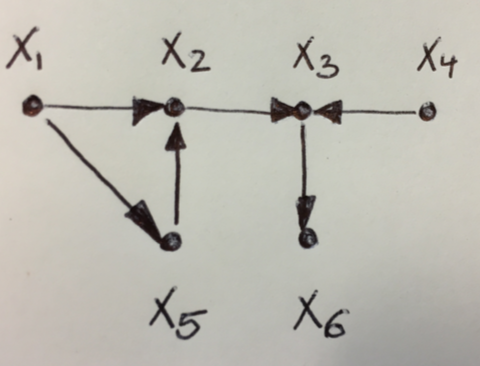
\includegraphics[width=0.5\linewidth]{figs/bayesnet.png}
\begin{itemize}
\item $X_1$ and $X_4$ are independent.
\item $X_1$ and $X_4$ are \textbf{not} independent given $X_6$.
\item $X_1$ and $X_4$ are independent given $X_2$.
\item $X_1$ and $X_4$ are independent given $X_2$ and $X_3$.
\item $X_1$ and $X_4$ are independent given $X_5$.
\end{itemize}

\subsection{Convex functions}
\begin{itemize}
\item $f(x) = x^{\alpha}, x \in \mathbb{R^+}, \forall \alpha \ge 1 or \le 0$
\item $f(x) = -x^3, x \in [-1,0]$
\item $f(x) = e^{ax}, \forall x,a \in \mathbb{R}$
\item $f(x) = ln(1/x), x \in \mathbb{R^+}$
\item $f(x) = g(h(x)), x \in \mathbb{R}, g,h$ convex and increasing over $\mathbb{R}$
\item $f(x) = ax+b, x \in \mathbb{R}, \forall a,b \in \mathbb{R}$
\item $f(x) = |x|^p, x \in \mathbb{R}, p\ge 1$
\item $f(x) = xlog(x), x \in \mathbb{R}^+$
\end{itemize}

\subsection{Non-convex functions}
\begin{itemize}
\item $f(x) = x^3, x \in [-1,1]$
\item $f(x) = e^{-x^/2}, x \in \mathbb{R}$
\item $\sum \mathcal{N}$
\item $sin(x) \forall x \in \mathbb{R}$
\end{itemize}
